\section{Sistema de Manufatura Didático}

\begin{frame}{Sistema de Manufatura Didático}
\begin{figure}[H]
  \centering
  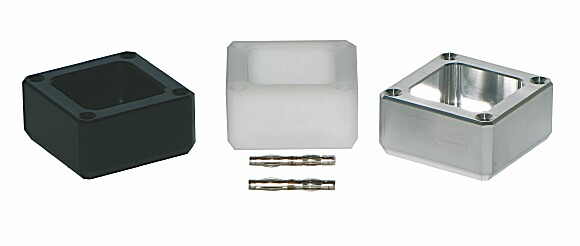
\includegraphics[width=0.5\textwidth]{maquete/pieces/workPieces.jpg}
  \caption{Cube halves.}
  \label{fig:cubeHalves}
\end{figure}
\end{frame}

\begin{frame}{Sistema de Manufatura Didático}
\centering
   \begin{figure}[ht]
\href{run:../../videos/timelapse.avi?start=75&stop=85}{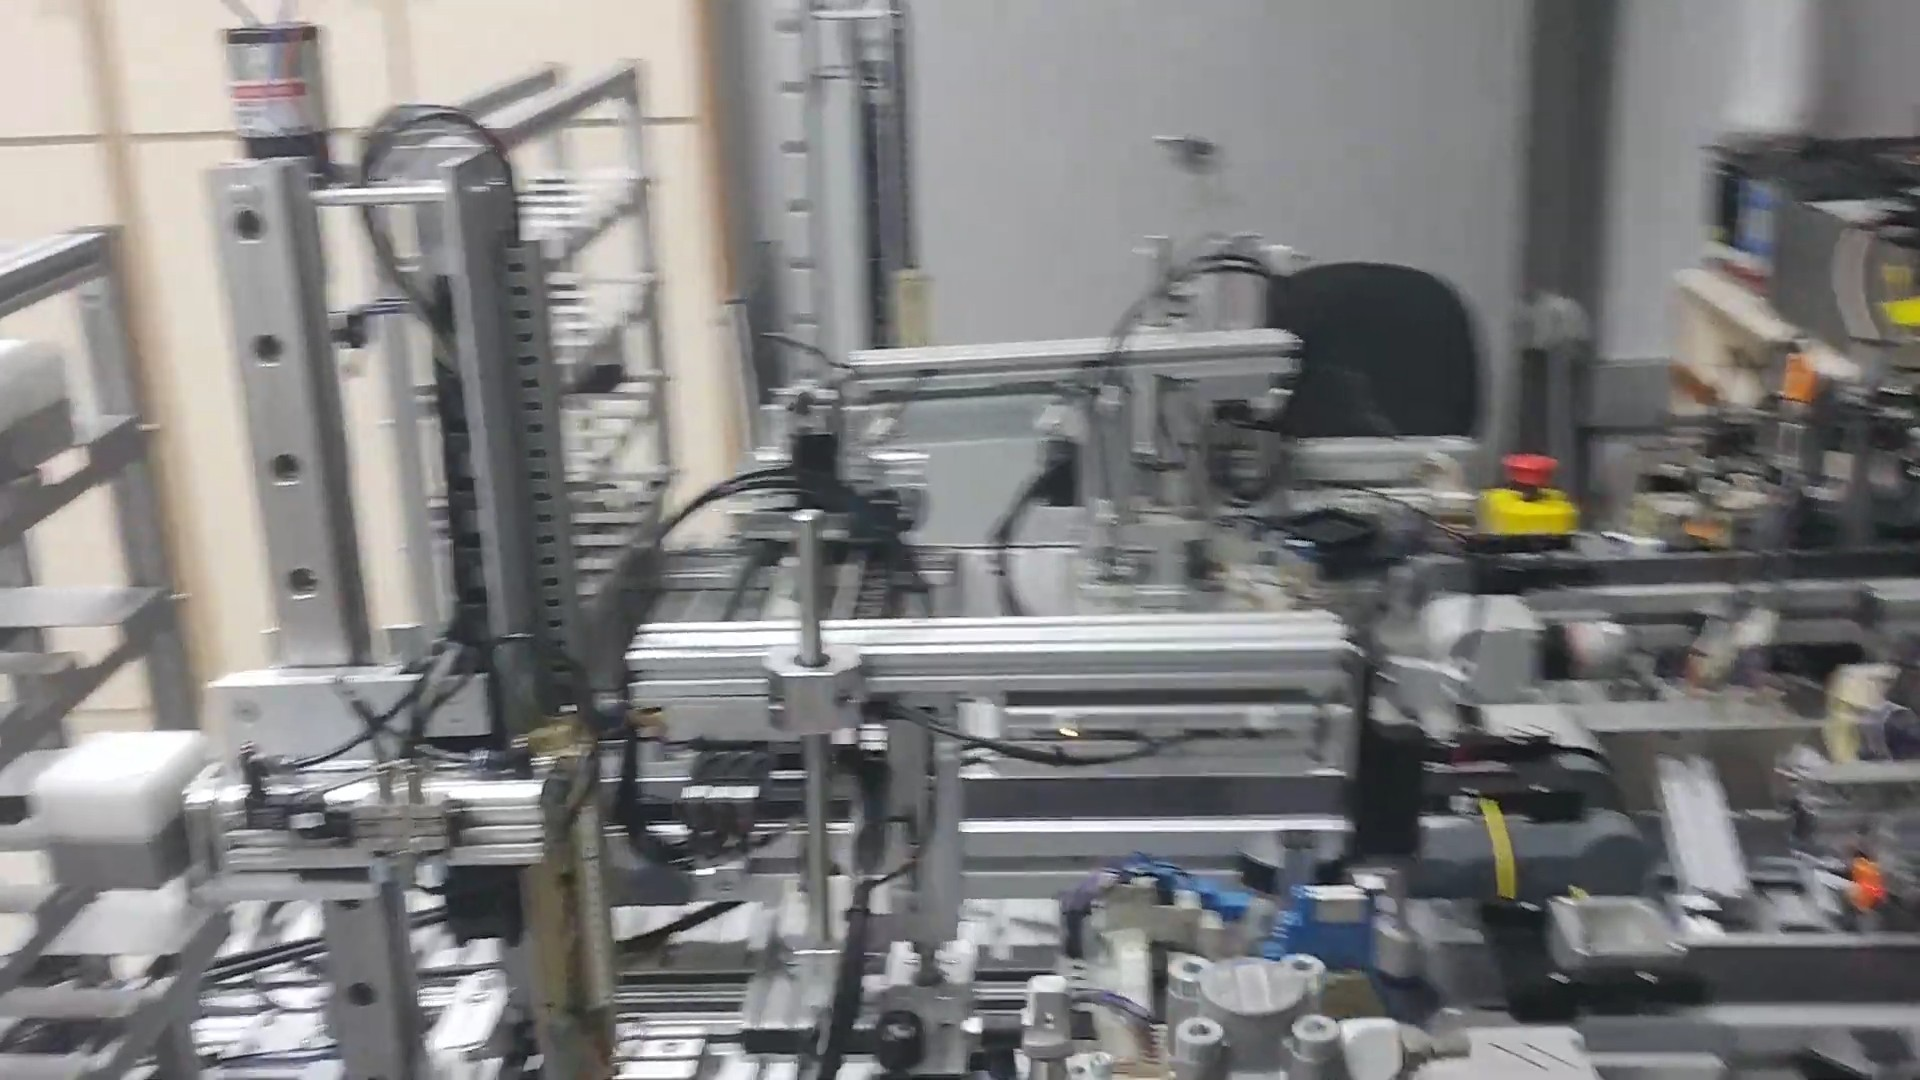
\includegraphics[width=0.7\textwidth]{../../videos/TCCVIDEO_cycle.jpg}}
\note{Exemplo de }
  \caption{Funcionamento da Planta.}
   \end{figure}
\end{frame}

\begin{frame}{Planta}
   \begin{figure}[ht]
       \begin{minipage}[b]{0.2\linewidth}
         \centering
  \includegraphics[width=\textwidth]{maquete/mag/mag.jpg}
       \end{minipage}
       \begin{minipage}[b]{0.2\linewidth}
         \centering
  \includegraphics[width=\textwidth]{maquete/esteira/esteira.jpg}
       \end{minipage}
       \begin{minipage}[b]{0.2\linewidth}
         \centering
  \includegraphics[width=\textwidth]{maquete/sensores/sensores.jpg}
\end{minipage}

\only<2>{
       \begin{minipage}[b]{0.2\linewidth}
         \centering
         PLC 1
  % \includegraphics[width=\textwidth]{maquete/braco/braco.jpg}
       \end{minipage}
       \vspace{0.3cm}
       \hrule
       ~\\

       \begin{minipage}[b]{0.2\linewidth}
         \centering
         PLC 2
       \end{minipage}
     }
     
       \begin{minipage}[b]{0.2\linewidth}
         \centering
  \includegraphics[width=\textwidth]{maquete/braco/braco.jpg}
       \end{minipage}
       \hspace{0.5cm}
       \begin{minipage}[b]{0.2\linewidth}
           \centering
  \includegraphics[width=\textwidth]{maquete/prensa/prensa.jpg}
       \end{minipage}
       \begin{minipage}[b]{0.2\linewidth}
           \centering
         \includegraphics[width=\textwidth]{maquete/elevador/elevador.jpg}
       \end{minipage}
  \caption{Módulos da Planta.}
   \end{figure}
\end{frame}
\begin{frame}{Rede de Petri implementada em múltiplos PLCs}
  \begin{figure}[ht]
       \begin{minipage}[b]{0.45\linewidth}
           \centering
           \includetikzfigure[width=\textwidth]{communicationPlcPN/communicationPlcPN}
           \caption{Rede de Petri no PLC 1.}
           \label{fig:a}
       \end{minipage}
       \hspace{0.5cm}
       \begin{minipage}[b]{0.45\linewidth}
           \centering
           \includetikzfigure[width=\textwidth]{communicationPlcPN/communicationPlcPN1}
           \caption{Rede de Petri no PLC 2.}
           \label{fig:b}
       \end{minipage}
  % \caption{Examplo de Rede de Petri implementeda em 2 PLCs.}
   \end{figure}
\end{frame}




\begin{frame}{Rede de Petri implementada em múltiplos PLCs}
   \begin{figure}[ht]
       \begin{minipage}[b]{0.45\linewidth}
         \centering
         \resizebox{0.8\textwidth}{!}{
           \adjustbox{trim=0pt 11cm 0 0,clip}{
           \includegraphics{communicationPlcPN/communicationPlcPNLadder.tikz}}}
       \end{minipage}
       \hspace{0.5cm}
       \begin{minipage}[b]{0.45\linewidth}
           \centering
           \resizebox{0.8\textwidth}{!}{
           \adjustbox{trim=0 0 0 11.5cm,clip}{
           \includegraphics{communicationPlcPN/communicationPlcPNLadder.tikz}}}
       \end{minipage}
  \caption{Diagrama Ladder de Rede de Petri no PLC 1.}
   \end{figure}
\end{frame}


\begin{frame}{Rede de Petri implementada em múltiplos PLCs}
   \begin{figure}[ht]
       \begin{minipage}[b]{0.45\linewidth}
         \centering
         \resizebox{0.8\textwidth}{!}{
           \adjustbox{trim=0pt 6.6cm 0 0,clip}{
           \includegraphics{communicationPlcPN/communicationPlcPN1Ladder.tikz}}}
       \end{minipage}
       \hspace{0.5cm}
       \begin{minipage}[b]{0.45\linewidth}
           \centering
           \resizebox{0.8\textwidth}{!}{
           \adjustbox{trim=0 0 0 8cm,clip}{
           \includegraphics{communicationPlcPN/communicationPlcPN1Ladder.tikz}}}
       \end{minipage}
  \caption{Diagrama Ladder de Rede de Petri no PLC 2.}
   \end{figure}
 \end{frame}

%%% Local Variables:
%%% mode: latex
%%% TeX-master: "../presentation"
%%% End:
